% General formatting
% \usepackage[hidelinks]{hyperref} % Hide colored links around references (needed for some conference templates like ICLR)
\usepackage[utf8]{inputenc} % From ACL template
\usepackage{times} % From ACL template
\usepackage{latexsym} % From ACL template
\usepackage[dvipsnames]{xcolor} % For color names
\usepackage{amsmath} % Extended math typesetting
\usepackage{amssymb} % Extended math symbols
\usepackage{mathtools} % More mathtools
\usepackage{annotate-equations} % Help annotate equations
\usepackage{pifont} % More symbols (also needed for checkmark and x-mark symbol macros)
\usepackage{truncate} % Help truncate text
\usepackage{enumitem} % allows setting leftmargin on \begin{enumerate} or \begin{itemize}
\usepackage{csquotes} % Inline and display quotes
\usepackage{xurl} % For \url
\usepackage[dont-mess-around]{fnpct} % Automatically ensures footnotes go after the punctuation mark
\usepackage{soul} % For text highlighting
% \usepackage{setspace} % Sometimes arXiV messes up line-spacing, this package can help correct it via \begin{spacing}{1.0}\end{spacing}

% Figure/Table Positioning
\usepackage{ragged2e} % allows \centering
\usepackage{float} % allows the [H] on \begin{figure}[H]

% Captions
\usepackage{caption}
\usepackage{subcaption} % For subfigures / captions: https://tex.stackexchange.com/a/122329

% Graphics
\usepackage{graphicx} % allows \includegraphics

% Tables
\usepackage{array}
\usepackage{longtable}
\usepackage{booktabs}
\usepackage{multirow}
\usepackage{arydshln}
\usepackage{tabularx}
\usepackage{tabulary}
\usepackage{makecell}

% Plots
\usepackage{tikz,pgfplots}
\pgfplotsset{compat=1.17}

% Loops and control flow in LaTeX
\usepackage{xinttools} % Useful to populate table data with a loop
\usepackage{ifthen} % If-then in LaTeX

% Placeholder content (Lorem Ipsum, etc.)
\usepackage{lipsum}

% Reviewing packages
\usepackage{todonotes}

% Render special character sets
% For proper rendering and hyphenation of words containing Latin characters (including in bib files)
\usepackage[T1]{fontenc}
% For Vietnamese characters
% \usepackage[T5]{fontenc}
% See https://www.latex-project.org/help/documentation/encguide.pdf for other character sets

% MACRO - Inline comment to comment out LaTeX code
\newcommand{\cmmnt}[1]{}

% MACRO - Visual annotations using todonotes, useful for review.
\newcommand{\note}[4][]{\todo[author=#2,color=#3,size=\scriptsize,#1]{#4}} % default note settings, used by macros below
\newcommand{\ajay}[2][]{\note[#1]{Ajay}{orange!40}{#2}} % Display in margins
\newcommand{\Ajay}[2][]{\ajay[inline,#1]{#2}} % Display inline

% MACRO - Checkmark and x-mark symbols
\newcommand{\cmark}{\ding{51}} % Checkmark symbol
\newcommand{\xmark}{\ding{55}} % X-mark symbol

% Import figures, tables, plots
\newcommand{\mainfig}{
    \begin{figure}[ht!]
        \centering
        \includegraphics[width=150px]{resources/figures/StyleDistanceNewSmall.png}
        \caption{\textsc{mStyleDistance} is trained using contrastive learning from synthetic positive and negative examples of \textasciitilde 40 style features in 9 languages to form both multilingual and cross-lingual training triplets.}
        \label{fig:main}
    \end{figure}
}

\newcommand{\mturkinterfacefig}{
    \begin{figure}[H]
        \centering
        \begin{subfigure}{0.85\linewidth}
            \centering
            \includegraphics[width=\linewidth]{resources/figures/mturkinterface1.png}
            \label{fig:mturkinterface1}
        \end{subfigure}
        \vspace{0.1cm}
        \begin{subfigure}{\linewidth}
            \centering
            \includegraphics[width=0.85\linewidth]{resources/figures/mturkinterface2.png}
            \label{fig:mturkinterface2}
        \end{subfigure}
        \caption{Instances from the annotation interface.}
        \label{fig:mturkinterface}
    \end{figure}
}

\newcommand{\stylefeaturecategoriesfig}{
    \begin{figure*}[ht!]
        \centering
        \resizebox{0.95\textwidth}{!}{
            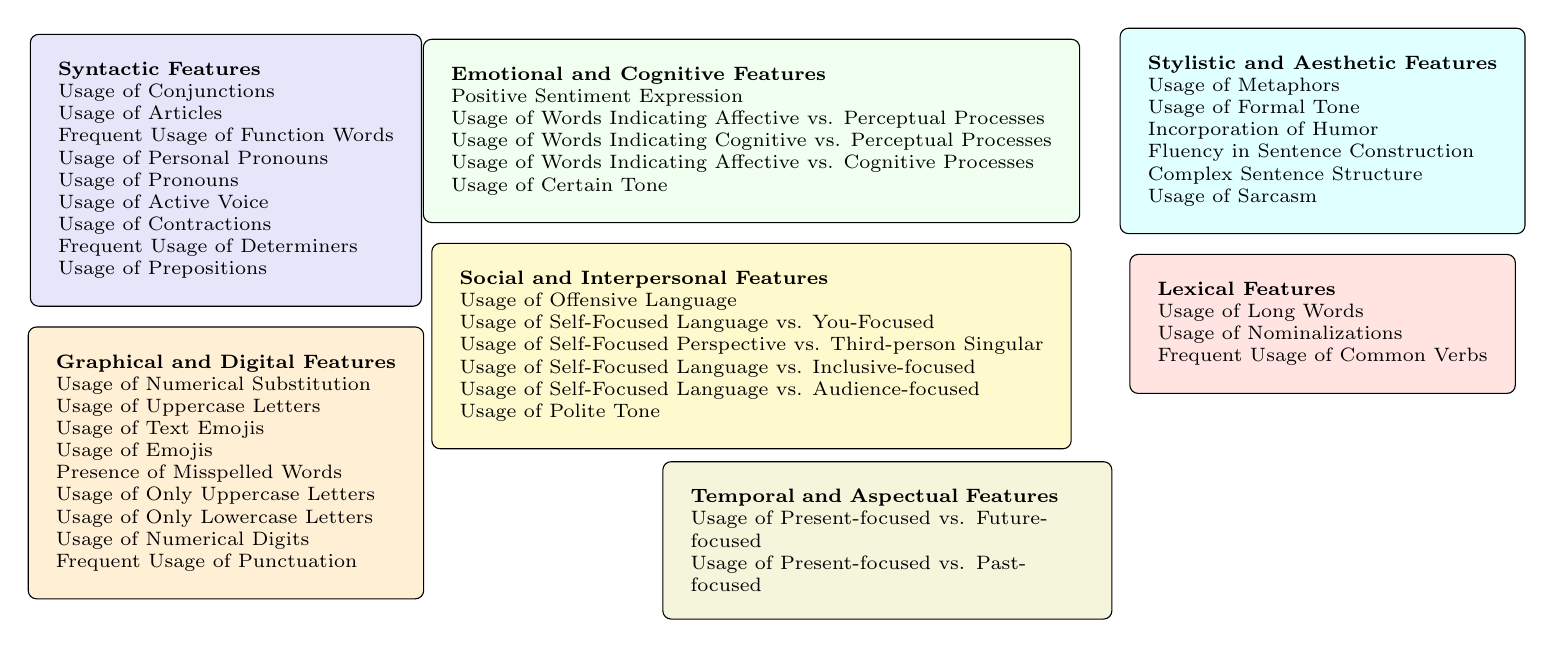
\begin{tikzpicture}[
                font=\scriptsize,
                category/.style={rectangle, draw, minimum width=4cm, inner sep=10pt, align=left, rounded corners=3pt}, % Same width within columns
                feature/.style={align=left}
            ]
            
            \definecolor{color1}{RGB}{230,230,250}  % Light lavender
            \definecolor{color2}{RGB}{255,239,213}  % Light peach
            \definecolor{color3}{RGB}{240,255,240}  % Light mint green
            \definecolor{color4}{RGB}{255,250,205}  % Light yellow
            \definecolor{color5}{RGB}{224,255,255}  % Light cyan
            \definecolor{color6}{RGB}{255,228,225}  % Light pink
            \definecolor{color7}{RGB}{245,245,220}  % Light beige
            \definecolor{color8}{RGB}{255,245,238}  % Light peach puff
            
            \node[category, fill=color1] (syntactic) at (-3, 0) {
                \textbf{Syntactic Features} \\ 
                Usage of Conjunctions \\
                Usage of Articles \\
                Frequent Usage of Function Words \\
                Usage of Personal Pronouns \\
                Usage of Pronouns \\
                Usage of Active Voice \\
                Usage of Contractions \\
                Frequent Usage of Determiners \\
                Usage of Prepositions
            };
            
            \node[category, fill=color2, below=0.25cm of syntactic] (graphical) {
                \textbf{Graphical and Digital Features} \\ 
                Usage of Numerical Substitution \\
                Usage of Uppercase Letters \\
                Usage of Text Emojis \\
                Usage of Emojis \\
                Presence of Misspelled Words \\
                Usage of Only Uppercase Letters \\
                Usage of Only Lowercase Letters \\
                Usage of Numerical Digits \\
                Frequent Usage of Punctuation
            };
            
            
            \node[category, fill=color3, right=0.5cm of syntactic] (emotional) at (-1, 0.5) {
                \textbf{Emotional and Cognitive Features} \\ 
                Positive Sentiment Expression \\
                Usage of Words Indicating Affective vs. Perceptual Processes \\
                Usage of Words Indicating Cognitive vs. Perceptual Processes \\
                Usage of Words Indicating Affective vs. Cognitive Processes \\
                Usage of Certain Tone
            };
    
            
            \node[category, fill=color5, right=0.5cm of emotional] (stylistic) {
                \textbf{Stylistic and Aesthetic Features} \\ 
                Usage of Metaphors \\
                Usage of Formal Tone \\
                Incorporation of Humor \\
                Fluency in Sentence Construction \\
                Complex Sentence Structure \\
                Usage of Sarcasm
            };
            
            \node[category, fill=color4, below=0.25cm of emotional] (social) {
                \textbf{Social and Interpersonal Features} \\ 
                Usage of Offensive Language \\
                Usage of Self-Focused Language vs. You-Focused \\
                Usage of Self-Focused Perspective vs. Third-person Singular\\
                Usage of Self-Focused Language vs. Inclusive-focused \\
                Usage of Self-Focused Language vs. Audience-focused  \\
                Usage of Polite Tone
            };
            
            
            \node[category, fill=color6, below=0.25cm of stylistic] (lexical) {
                \textbf{Lexical Features} \\ 
                Usage of Long Words \\
                Usage of Nominalizations \\
                Frequent Usage of Common Verbs
            };
            
            \node[category, fill=color7, text width=5cm] (temporal) at (5.4, -4.7) {
                \textbf{Temporal and Aspectual Features} \\ 
                Usage of Present-focused vs. Future-focused \\
                Usage of Present-focused vs. Past-focused
            };
            
            \end{tikzpicture}
        }
        \caption{We generate synthetic parallel examples to train \textsc{StyleDistance} for a wide range of style features in seven linguistic and stylistic categories. Further details on these features can be found in Appendix \ref{sec:appendix:stylefeatures}.}
        \label{fig:stylefeaturecategories}
    \end{figure*}
}



\newcommand{\stelfig}{
    \begin{figure*}[htbp]
        \centering
        \includegraphics[width=215px]{resources/figures/STELFigure.png}
        % \begin{tikzpicture}
        %     \node[rectangle,
        %         draw = lightgray,
        %         text = black,
        %         fill = lightgray,
        %         minimum width = 215px, 
        %         minimum height = 270px] (r) at (0,0) {Main Figure};
        % \end{tikzpicture}
        \caption{A visualization of the STEL and STEL-or-Content task evaluation we describe in Section \ref{sec:steleval}.}
        \label{fig:stel}
    \end{figure*}
}

\newcommand{\multilingualstelorcontentfig}{
    \begin{figure}[H]
        \centering
        \includegraphics[width=.6\linewidth]{resources/figures/multilingual-stel-or-content.png}
        \caption{Instance from our multilingual STEL-or-Content benchmark.} %, anchor 1 (A1) has the same content but different style from sentence 1 (S1) and the same style but different content from sentence 2 (S2). Both the anchor and the two sentences are in the same language. The task is to successfully pair A1 and S2 together rather than A1 and S1.}
        \label{fig:multilingualstelorcontent}
    \end{figure}
}

\newcommand{\crosslingualstelorcontentfig}{
    \begin{figure}[H]
        \centering
        \includegraphics[width=.6\linewidth]{resources/figures/crosslingual-stel-or-content.png}
        \caption{Instance from our cross-lingual STEL-or-Content benchmark.} % has the same setup as multilingual STEL-or-content except the two sentences are in a different language than the anchor.}
        \label{fig:crosslingualstelorcontent}
    \end{figure}
}


\newcommand{\stelevaltable}{
    \begin{table*}[!h]
    \centering
    \large
    % \resizebox{\textwidth}{!}{
    \scalebox{0.75}{
    \begin{tabular}{l*{5}{c}}
    \toprule[\heavyrulewidth]
    \textbf{Model} 
    & \textbf{Simplicity} 
    & \textbf{Formality} 
    & \textbf{Toxicity} 
    & \textbf{Positivity} 
    & \textbf{Formality (cross-lingual)} \\ \midrule
    \textbf{\citet{styleemb}} 
    & 0.23 
    & 0.63 
    & 0.19 
    & 0.23 
    & 0.45 \\ 
    \textbf{\textsc{StyleDistance}} 
    & 0.21 
    & 0.67 
    & 0.15 
    & 0.18 
    & 0.49 \\ 
    \textbf{xlm-roberta-base} 
    & 0.12 
    & 0.16 
    & 0.09 
    & 0.07 
    & 0.19 \\ 
    \textbf{LISA} 
    & 0.15 
    & 0.09 
    & 0.09 
    & 0.21 
    & 0.27 \\ 
    \textbf{\textsc{mStyleDistance}} 
    & \textbf{0.36} 
    & \textbf{0.71} 
    & \textbf{0.37} 
    & \textbf{0.30} 
    & \textbf{0.53} \\ 
    \bottomrule[\heavyrulewidth]
    \end{tabular}
    }
    \caption{Performance on the multilingual and cross-lingual STEL-or-content benchmarks, averaged across languages for each style feature. \textsc{mStyleDistance} leads in cross-lingual and overall performance.}
    \label{table:steleval}
    \end{table*}
}

% \newcommand{\stelevalfull}{
%     \begin{table*}[!h]
%     \centering
%     \small
%     \begin{tabular}{lrrrrr}
%     \toprule[\heavyrulewidth]
%     \textbf{Language} & \textbf{\citet{styleemb}} & \textbf{\textsc{StyleDistance}} & \textbf{xlm-roberta-base} & \textbf{LISA} & \textbf{\textsc{mStyleDistance}} \\
%     \midrule
%     \multicolumn{6}{l}{\textbf{Simplicity}} \\
%     de      & 0.23   & 0.06   & 0.00   & 0.00   & 0.24    \\
%     en      & 0.26   & 0.32   & 0.05   & 0.00   & 0.36    \\
%     fr      & 0.29   & 0.33   & 0.22   & 0.12   & 0.46    \\
%     it      & 0.21   & 0.15   & 0.08   & 0.03   & 0.48    \\
%     ja      & 0.09   & 0.05   & 0.01   & 0.48   & 0.14    \\
%     pt-br   & 0.10   & 0.07   & 0.04   & 0.03   & 0.15    \\
%     ru      & 0.26   & 0.24   & 0.07   & 0.15   & 0.38    \\
%     sl      & 0.43   & 0.43   & 0.46   & 0.39   & 0.69    \\
%     average & 0.23   & 0.21   & 0.12   & 0.15   & 0.36    \\
%     \midrule
%     \multicolumn{6}{l}{\textbf{Formality}} \\
%     fr      & 0.70   & 0.81   & 0.16   & 0.06   & 0.82    \\
%     it      & 0.64   & 0.63   & 0.18   & 0.10   & 0.69    \\
%     pt-br   & 0.56   & 0.57   & 0.15   & 0.11   & 0.62    \\
%     average & 0.63   & 0.67   & 0.16   & 0.09   & 0.71    \\
%     \midrule
%     \multicolumn{6}{l}{\textbf{Toxicity}} \\
%     am      & 0.35   & 0.29   & 0.24   & 0.21   & 0.53    \\
%     ar      & 0.05   & 0.04   & 0.02   & 0.10   & 0.18    \\
%     de      & 0.01   & 0.02   & 0.01   & 0.00   & 0.28    \\
%     en      & 0.56   & 0.48   & 0.09   & 0.08   & 0.51    \\
%     es      & 0.26   & 0.20   & 0.13   & 0.05   & 0.35    \\
%     hi      & 0.15   & 0.09   & 0.09   & 0.15   & 0.37    \\
%     ru      & 0.18   & 0.16   & 0.13   & 0.09   & 0.61    \\
%     uk      & 0.07   & 0.05   & 0.04   & 0.02   & 0.25    \\
%     zh      & 0.05   & 0.02   & 0.04   & 0.07   & 0.23    \\
%     average & 0.19   & 0.15   & 0.09   & 0.09   & 0.37    \\
%     \midrule
%     \multicolumn{6}{l}{\textbf{Positivity}} \\
%     bn      & 0.27   & 0.13   & 0.04   & 0.23   & 0.32    \\
%     en      & 0.21   & 0.20   & 0.03   & 0.19   & 0.18    \\
%     hi      & 0.11   & 0.10   & 0.04   & 0.14   & 0.22    \\
%     mag     & 0.09   & 0.08   & 0.08   & 0.13   & 0.41    \\
%     ml      & 0.32   & 0.28   & 0.10   & 0.27   & 0.39    \\
%     mr      & 0.19   & 0.18   & 0.03   & 0.17   & 0.22    \\
%     or      & 0.27   & 0.19   & 0.08   & 0.24   & 0.35    \\
%     pa      & 0.18   & 0.15   & 0.06   & 0.17   & 0.23    \\
%     te      & 0.39   & 0.34   & 0.20   & 0.29   & 0.40    \\
%     ur      & 0.24   & 0.20   & 0.08   & 0.28   & 0.26    \\
%     average & 0.23   & 0.18   & 0.07   & 0.21   & 0.30    \\
%     \midrule
%     \multicolumn{6}{l}{\textbf{Formality (crosslingual)}} \\
%     fr-it  & 0.47   & 0.51   & 0.27   & 0.22   & 0.53    \\
%     fr-pt  & 0.45   & 0.48   & 0.25   & 0.19   & 0.52    \\
%     it-fr  & 0.48   & 0.53   & 0.30   & 0.18   & 0.53    \\
%     it-pt  & 0.41   & 0.45   & 0.24   & 0.19   & 0.52    \\
%     pt-fr  & 0.46   & 0.53   & 0.30   & 0.17   & 0.53    \\
%     pt-it  & 0.42   & 0.47   & 0.29   & 0.21   & 0.52    \\
%     average & 0.45   & 0.49   & 0.28   & 0.19   & 0.53    \\
%     \bottomrule
%     \end{tabular}
%     \caption{Full performance on the multilingual and crosslingual STEL-or-content benchmarks. For the crosslingual SoC evaluation, "a-b" means that the anchor sentences were all in language a and alternative sentences were all in language b. \textsc{mStyleDistance} leads in crosslingual and overall performance.}
%     \end{table*}
% }
\newcommand{\stelevalfull}{
    \begin{table*}[!h]
    \centering
    \small
    \begin{tabularx}{\textwidth}{l *{5}{>{\centering\arraybackslash}X}}
    \toprule[\heavyrulewidth]
    \textbf{Language} & \textbf{\citet{styleemb}} & \textbf{\textsc{StyleDistance}} & \textbf{xlm-roberta-base} & \textbf{LISA} & \textbf{\textsc{mStyleDistance}} \\
    \midrule
    \multicolumn{6}{l}{\textbf{Simplicity}} \\ \midrule
    de      & 0.23   & 0.06   & 0.00   & 0.00   & \textbf{0.24}    \\
    en      & 0.26   & 0.32   & 0.05   & 0.00   & \textbf{0.36}    \\
    fr      & 0.29   & 0.33   & 0.22   & 0.12   & \textbf{0.46}    \\
    it      & 0.21   & 0.15   & 0.08   & 0.03   & \textbf{0.48}    \\
    ja      & 0.09   & 0.05   & 0.01   & \textbf{0.48}   & 0.14    \\
    pt-br   & 0.10   & 0.07   & 0.04   & 0.03   & \textbf{0.15}    \\
    ru      & 0.26   & 0.24   & 0.07   & 0.15   & \textbf{0.38}    \\
    sl      & 0.43   & 0.43   & 0.46   & 0.39   & \textbf{0.69}    \\
    \midrule
    average & 0.23   & 0.21   & 0.12   & 0.15   & \textbf{0.36}    \\
    \midrule
    \multicolumn{6}{l}{\textbf{Formality}} \\ \midrule
    fr      & 0.70   & 0.81   & 0.16   & 0.06   & \textbf{0.82}    \\
    it      & 0.64   & 0.63   & 0.18   & 0.10   & \textbf{0.69}    \\
    pt-br   & 0.56   & 0.57   & 0.15   & 0.11   & \textbf{0.62}    \\
    \midrule
    average & 0.63   & 0.67   & 0.16   & 0.09   & \textbf{0.71}    \\
    \midrule
    \multicolumn{6}{l}{\textbf{Toxicity}} \\ \midrule
    am      & 0.35   & 0.29   & 0.24   & 0.21   & \textbf{0.53}    \\
    ar      & 0.05   & 0.04   & 0.02   & 0.10   & \textbf{0.18}    \\
    de      & 0.01   & 0.02   & 0.01   & 0.00   & \textbf{0.28}    \\
    en      & \textbf{0.56}   & 0.48   & 0.09   & 0.08   & 0.51    \\
    es      & 0.26   & 0.20   & 0.13   & 0.05   & \textbf{0.35}    \\
    hi      & 0.15   & 0.09   & 0.09   & 0.15   & \textbf{0.37}    \\
    ru      & 0.18   & 0.16   & 0.13   & 0.09   & \textbf{0.61}    \\
    uk      & 0.07   & 0.05   & 0.04   & 0.02   & \textbf{0.25}    \\
    zh      & 0.05   & 0.02   & 0.04   & 0.07   & \textbf{0.23}    \\
    \midrule
    average & 0.19   & 0.15   & 0.09   & 0.09   & \textbf{0.37}    \\
    \midrule
    \multicolumn{6}{l}{\textbf{Positivity}} \\ \midrule
    bn      & 0.27   & 0.13   & 0.04   & 0.23   & \textbf{0.32}    \\
    en      & \textbf{0.21}   & 0.20   & 0.03   & 0.19   & 0.18    \\
    hi      & 0.11   & 0.10   & 0.04   & 0.14   & \textbf{0.22}    \\
    mag     & 0.09   & 0.08   & 0.08   & 0.13   & \textbf{0.41}    \\
    ml      & 0.32   & 0.28   & 0.10   & 0.27   & \textbf{0.39}    \\
    mr      & 0.19   & 0.18   & 0.03   & 0.17   & \textbf{0.22}     \\
    or      & 0.27   & 0.19   & 0.08   & 0.24   & \textbf{0.35}    \\
    pa      & 0.18   & 0.15   & 0.06   & 0.17   & \textbf{0.23}    \\
    te      & 0.39   & 0.34   & 0.20   & 0.29   & \textbf{0.40}    \\
    ur      & 0.24   & 0.20   & 0.08   & 0.28   & \textbf{0.26}    \\
    \midrule
    average & 0.23   & 0.18   & 0.07   & 0.21   & \textbf{0.30}    \\
    \midrule
    \multicolumn{6}{l}{\textbf{Formality (cross-lingual)}} \\ \midrule
    fr-it  & 0.47   & 0.51   & 0.22   & 0.28   & \textbf{0.53}    \\
    fr-pt  & 0.45   & 0.48   & 0.19   & 0.29   & \textbf{0.52}    \\
    it-fr  & 0.48   & \textbf{0.53}   & 0.18   & 0.26   & \textbf{0.53}    \\
    it-pt  & 0.41   & 0.45   & 0.19   & 0.27   & \textbf{0.52}    \\
    pt-fr  & 0.46   & \textbf{0.53}   & 0.17   & 0.27   & \textbf{0.53}    \\
    pt-it  & 0.42   & 0.47   & 0.21   & 0.27   & \textbf{0.52}    \\
    \midrule
    average & 0.45   & 0.49   & 0.19   & 0.27   & \textbf{0.53}    \\
    \bottomrule
    \end{tabularx}
    \caption{Full performance on the multilingual and cross-lingual STEL-or-content benchmarks. For the cross-lingual SoC evaluation, "a-b" means that the anchor sentences were all in language a and alternative sentences were all in language b. \textsc{mStyleDistance} leads in cross-lingual and overall performance.}
    \end{table*}
}

\newcommand{\synthstelevaltable}{
    \begin{table}[!t]
    \centering
    \small
    \begin{tabular}{>{\raggedright\arraybackslash}p{.3\textwidth}cc}
    \toprule
    \textbf{Model} & \textbf{STEL} & \textbf{S-o-C} \\
    \midrule
    LISA & 0.79 & 0.06 \\
    \citet{styleemb} & 0.76 & 0.25 \\
    % \textsc{StyleDistance} & \textbf{0.88} & \textbf{0.97} \\
    % $\textsc{StyleDistance}_{\textsc{Synth}}$ & 0.74 & 0.89 \\
    \bottomrule
    \end{tabular}
    \caption{Results obtained by LISA and the \citet{styleemb} embeddings on STEL and STEL-or-Content instances created from the test split of our \textsc{SynthStel} dataset. 
     %Results on STEL/STEL-or-Content task instances created using the test split of our \textsc{SynthStel} synthetic dataset in order to probe how well LISA and \citet{styleemb} capture the 40 style features we use in training \textsc{StyleDistance} models. 
    See Appendix \ref{sec:appendix:fullsynthstelresults} for full results.}
    \label{table:synthsteleval}
    \end{table}
}

\newcommand{\fullsynthstelevaltable}{
\begingroup
\hyphenpenalty=100000000
\exhyphenpenalty=100000000

    \begin{table*}[!h]
    \centering
    \small
    \setlength{\tabcolsep}{4pt}
    \resizebox{\textwidth}{!}{
    \begin{tabular}{>{\raggedright\arraybackslash}p{.3\textwidth}*{3}{c}c|*{4}{c}}
    \toprule
    \textbf{Style Feature} 
    & \multicolumn{2}{c}{LISA} 
    & \multicolumn{2}{c}{\citet{styleemb}} 
    & \multicolumn{2}{c}{\textsc{StyleDistance}} 
    & \multicolumn{2}{c}{$\textsc{StyleDistance}_{\textsc{Synth}}$} \\ \cmidrule(lr){2-3} \cmidrule(lr){4-5} \cmidrule(lr){6-7} \cmidrule(lr){8-9}
    & \textbf{STEL} & \textbf{S-o-C}
    & \textbf{STEL} & \multicolumn{1}{c}{\textbf{S-o-C}}
    & \textbf{STEL} & \textbf{S-o-C}
    & \textbf{STEL} & \textbf{S-o-C} \\
    \midrule
    Usage of Polite Tone & 0.93 & 0.18 & 0.76 & 0.53 & 1.00 & 1.00 & 0.78 & 1.00 \\
    Incorporation of Humor & 0.78 & 0.27 & 0.76 & 0.31 & 1.00 & 1.00 & 0.82 & 0.89 \\
    Usage of Sarcasm & 0.60 & 0.04 & 0.87 & 0.11 & 0.98 & 1.00 & 0.53 & 0.56 \\
    Usage of Metaphors & 0.91 & 0.02 & 0.53 & 0.16 & 0.98 & 0.73 & 0.58 & 0.82 \\
    Usage of Offensive Language & 1.00 & 0.40 & 0.80 & 0.13 & 1.00 & 1.00 & 0.49 & 0.93 \\
    Positive Sentiment Expression & 1.00 & 0.51 & 0.51 & 0.04 & 0.96 & 1.00 & 0.47 & 0.53 \\
    Usage of Active Voice & 0.64 & 0.00 & 0.64 & 0.07 & 1.00 & 1.00 & 0.91 & 1.00 \\
    Usage of Certain Tone & 1.00 & 0.20 & 0.60 & 0.00 & 0.87 & 1.00 & 0.87 & 0.93 \\
    Usage of Self-Focused Language vs. Inclusive-focused & 0.87 & 0.00 & 0.64 & 0.00 & 0.76 & 1.00 & 0.69 & 0.89 \\
    Usage of Self-Focused Language vs. You-Focused & 0.96 & 0.00 & 0.73 & 0.04 & 0.78 & 1.00 & 0.60 & 0.80 \\
    Usage of Self-Focused Language vs. Audience-focused & 0.73 & 0.00 & 1.00 & 0.16 & 0.91 & 1.00 & 0.67 & 1.00 \\
    Usage of Self-Focused Perspective vs. Third-person Singular & 0.76 & 0.00 & 0.44 & 0.02 & 0.73 & 1.00 & 0.60 & 0.82 \\
    Usage of Personal Pronouns & 0.64 & 0.00 & 0.56 & 0.04 & 0.82 & 1.00 & 0.80 & 0.78 \\
    Usage of Present-focused vs. Future-focused & 1.00 & 0.00 & 0.56 & 0.02 & 0.58 & 1.00 & 0.62 & 0.80 \\
    Usage of Present-focused vs. Past-focused & 0.89 & 0.00 & 0.60 & 0.04 & 0.89 & 1.00 & 0.47 & 0.91 \\
    Usage of Words Indicating Affective vs. Cognitive Processes & 1.00 & 0.07 & 0.87 & 0.09 & 0.64 & 1.00 & 0.69 & 1.00 \\
    Usage of Words Indicating Affective vs. Perceptual Processes & 0.69 & 0.02 & 0.67 & 0.00 & 1.00 & 1.00 & 1.00 & 1.00 \\
    Usage of Words Indicating Cognitive vs. Perceptual Processes & 0.76 & 0.04 & 0.56 & 0.04 & 0.91 & 1.00 & 0.71 & 0.69 \\
    Usage of Articles & 0.69 & 0.00 & 0.69 & 0.02 & 0.89 & 1.00 & 0.82 & 0.93 \\
    Fluency in Sentence Construction & 0.60 & 0.00 & 0.91 & 0.62 & 0.98 & 1.00 & 1.00 & 1.00 \\
    Frequent Usage of Function Words & 0.58 & 0.02 & 0.56 & 0.24 & 0.82 & 1.00 & 0.80 & 0.96 \\
    Frequent Usage of Common Verbs & 0.67 & 0.00 & 0.82 & 0.07 & 0.78 & 0.89 & 0.49 & 0.89 \\
    Usage of Pronouns & 0.96 & 0.00 & 0.53 & 0.24 & 0.78 & 1.00 & 0.62 & 0.80 \\
    Usage of Prepositions & 0.67 & 0.00 & 0.78 & 0.13 & 0.73 & 1.00 & 0.82 & 0.71 \\
    Frequent Usage of Determiners & 0.53 & 0.00 & 0.69 & 0.07 & 0.93 & 1.00 & 0.53 & 0.98 \\
    Usage of Conjunctions & 0.49 & 0.00 & 0.64 & 0.31 & 0.67 & 1.00 & 0.67 & 0.96 \\
    Usage of Nominalizations & 0.58 & 0.00 & 0.96 & 0.07 & 0.80 & 1.00 & 0.56 & 1.00 \\
    Usage of Long Words & 1.00 & 0.00 & 0.91 & 0.44 & 1.00 & 1.00 & 0.64 & 0.91 \\
    Usage of Numerical Digits & 0.58 & 0.00 & 0.58 & 0.02 & 0.93 & 0.80 & 0.58 & 0.62 \\
    Usage of Uppercase Letters & 0.78 & 0.00 & 1.00 & 0.98 & 1.00 & 1.00 & 1.00 & 1.00 \\
    Frequent Usage of Punctuation & 0.56 & 0.00 & 0.93 & 0.58 & 0.78 & 1.00 & 0.67 & 0.80 \\
    Usage of Formal Tone & 0.89 & 0.00 & 0.98 & 0.36 & 1.00 & 1.00 & 0.64 & 0.98 \\
    Complex Sentence Structure & 0.56 & 0.00 & 0.60 & 0.16 & 0.51 & 0.76 & 0.73 & 0.87 \\
    Usage of Contractions & 0.71 & 0.02 & 1.00 & 0.31 & 1.00 & 0.89 & 1.00 & 0.93 \\
    Usage of Numerical Substitution & 0.81 & 0.00 & 0.90 & 0.04 & 0.90 & 0.87 & 0.90 & 1.00 \\
    Usage of Only Lowercase Letters & 0.89 & 0.00 & 1.00 & 1.00 & 1.00 & 1.00 & 1.00 & 1.00 \\
    Usage of Only Uppercase Letters & 0.98 & 0.33 & 0.87 & 0.18 & 1.00 & 1.00 & 1.00 & 1.00 \\
    Presence of Misspelled Words & 1.00 & 0.24 & 1.00 & 0.91 & 1.00 & 1.00 & 1.00 & 0.96 \\
    Usage of Text Emojis & 1.00 & 0.02 & 0.91 & 0.78 & 1.00 & 1.00 & 1.00 & 1.00 \\
    Usage of Emojis & 1.00 & 0.00 & 1.00 & 0.47 & 1.00 & 1.00 & 1.00 & 1.00 \\
    \midrule
    \textbf{Average} & 0.79 & 0.06 & 0.76 & 0.25 & 0.88 & 0.97 & 0.74 & 0.89 \\
    \bottomrule
    \end{tabular}
    }
    \caption{STEL and STEL-or-Content results for top-performing models on the \textsc{SynthStel} test split. This table shows the performance variations and coverage of LISA and \citet{styleemb} embeddings for the 40 different style features found in the dataset. After training \textsc{StyleDistance} models on the \textsc{SynthStel} train split, we observe strong coverage of these 40 style features as expected, demonstrating the successful distillation of the LLM's strong style knowledge into a more efficient representation model \citep{distillation}.}
    \label{table:fullsynthsteleval}
    \end{table*}
\endgroup
}
% \begin{table}[!t]
% \centering
% \scalebox{0.68}{
%     \begin{tabular}{ll cccc}
%       \toprule
%       & \multicolumn{4}{c}{\textbf{Intellipro Dataset}}\\
%       & \multicolumn{2}{c}{Rank Resume} & \multicolumn{2}{c}{Rank Job} \\
%       \cmidrule(lr){2-3} \cmidrule(lr){4-5} 
%       \textbf{Method}
%       &  Recall@100 & nDCG@100 & Recall@10 & nDCG@10 \\
%       \midrule
%       \confitold{}
%       & 71.28 &34.79 &76.50 &52.57 
%       \\
%       \cmidrule{2-5}
%       \confitsimple{}
%     & 82.53 &48.17
%        & 85.58 &64.91
     
%        \\
%        +\RunnerUpMiningShort{}
%     &85.43 &50.99 &91.38 &71.34 
%       \\
%       +\HyReShort
%         &- & -
%        &-&-\\
       
%       \bottomrule

%     \end{tabular}
%   }
% \caption{Ablation studies using Jina-v2-base as the encoder. ``\confitsimple{}'' refers using a simplified encoder architecture. \framework{} trains \confitsimple{} with \RunnerUpMiningShort{} and \HyReShort{}.}
% \label{tbl:ablation}
% \end{table}
\begin{table*}[!t]
\centering
\scalebox{0.75}{
    \begin{tabular}{l cccc cccc}
      \toprule
      & \multicolumn{4}{c}{\textbf{Recruiting Dataset}}
      & \multicolumn{4}{c}{\textbf{AliYun Dataset}}\\
      & \multicolumn{2}{c}{Rank Resume} & \multicolumn{2}{c}{Rank Job} 
      & \multicolumn{2}{c}{Rank Resume} & \multicolumn{2}{c}{Rank Job}\\
      \cmidrule(lr){2-3} \cmidrule(lr){4-5} 
      \cmidrule(lr){6-7} \cmidrule(lr){8-9} 
      \textbf{Method}
      & Recall@100 & nDCG@100 & Recall@10 & nDCG@10
      & Recall@100 & nDCG@100 & Recall@10 & nDCG@10\\
      \midrule
      \confitold{}
      & 71.28 & 34.79 & 76.50 & 52.57 
      & 87.81 & 65.06 & 72.39 & 56.12
      \\
      \cmidrule{2-9}
      \confitsimple{}
      & 82.53 & 48.17 & 85.58 & 64.91
      & 94.90&78.40 & 78.70& 65.45
       \\
      +\HyReShort{}
       &85.28 & 49.50
       &90.25 & 70.22
       & 96.62&81.99 & \textbf{81.16}& 67.63
       \\
      +\RunnerUpMiningShort{}
       % & 85.14& 49.82
       % &90.75&72.51
       & \textbf{86.13}&\textbf{51.90} & \textbf{94.25}&\textbf{73.32}
       & \textbf{97.07}&\textbf{83.11} & 80.49& \textbf{68.02}
       \\
   %     +\RunnerUpMiningShort{}
   %    & 85.43 & 50.99 & 91.38 & 71.34 
   %    & 96.24 & 82.95 & 80.12 & 66.96
   %    \\
   %    +\HyReShort{} old
   %     &85.28 & 49.50
   %     &90.25 & 70.22
   %     & 96.62&81.99 & 81.16& 67.63
   %     \\
   % +\HyReShort{} 
   %     % & 85.14& 49.82
   %     % &90.75&72.51
   %     & 86.83&51.77 &92.00 &72.04
   %     & 97.07&83.11 & 80.49& 68.02
   %     \\
      \bottomrule

    \end{tabular}
  }
\caption{\framework{} ablation studies. ``\confitsimple{}'' refers using a simplified encoder architecture. \framework{} trains \confitsimple{} with \RunnerUpMiningShort{} and \HyReShort{}. We use Jina-v2-base as the encoder due to its better performance.
}
\label{tbl:ablation}
\end{table*}
\newcommand{\ablationsimpletable}{
    \begin{table}[!h]
    \centering
    \small
    \setlength{\tabcolsep}{3pt}
    \begin{tabular}{l|c|c|c|c}
    \toprule[\heavyrulewidth]
     \multirow{2}{*}{\textbf{Features Tested}}
    & \multirow{2}{*}{\textbf{m avg}}
    & \multirow{2}{*}{\textbf{c avg}}
    &  \multicolumn{2}{c}{\textbf{Retained Perf (\%)}} \\ 
    & & & ~~~~ m ~~~~ & c \\ \midrule
    In-Domain
    & 0.38
    & 0.53
    & 100\% & 100\% \\
    Out of Domain
    & 0.31
    & 0.44
    & 75\% & 74\% \\
    Out of Distribution
    & 0.31
    & 0.40
    & 75\% & 62\% \\
    No Language Overlap
    & 0.35
    & 0.52
    & 89\% & 97\% \\
    \bottomrule[\heavyrulewidth]
    \end{tabular}
    \caption{\textsc{mStyleDistance} embeddings under three generalization conditions on the multilingual (m avg) and cross-lingual (c avg) STEL-or-Content tasks.}
    \label{table:simplifiedablation}
    \end{table}
}

\newcommand{\stylefeaturestable}{
    {
    \tiny
    \renewcommand{\arraystretch}{2} % Adds space between rows
    \begin{longtable}{p{3cm} p{3cm} p{6.5cm} p{2cm}}
      \toprule
      \textbf{Style Feature} & \textbf{Positive and Negative Prompts} & \textbf{Style Feature Definition} & \textbf{Excluded In} \\
      \midrule
      \endfirsthead
    
      \toprule
      \textbf{Style Feature Name} & \textbf{Positive and Negative Prompts} & \textbf{Style Feature Definition} & \textbf{Excluded In} \\
      \midrule
      \endhead
    
      \bottomrule
      \endfoot
    
      \bottomrule
      \addlinespace
      \caption{40 style features, with the `Excluded in' column indicating that a particular feature was omitted from our dataset due to its inapplicability to a specific language.}
      \label{table:stylefeaturestable} \\
      \endlastfoot
    
      % Add your table rows below this line

% Usage of Articles & Positive: With articles \newline Negative: Less frequent articles & The "Usage of Articles" text style feature refers to how often a text uses words like "a", "an", and "the". These words are called articles and they are used before nouns. This feature measures the frequency of these articles in a given text. & Arabic, Hindi, Japanese, Korean, Russian, Chinese\\
% Usage of Long Words & Positive: Long average word length \newline Negative: Short average word length & The "Usage of Long Words" text style feature refers to the frequency or prevalence of long words, typically those with more than six or seven letters, in a given text. This style feature is often used to measure the complexity or sophistication of the text. If a text has many long words, it is said to have a high usage of long words. & Arabic, Japanese, Korean, Chinese\\
% Usage of Uppercase Letters & Positive: With uppercase letters \newline Negative: Without uppercase letters & The usage of uppercase letters as a text style feature refers to the frequency or manner in which capital letters are used in a text. This could be for emphasis, to denote shouting or strong emotions, or to highlight specific words or phrases. It's not just about the start of sentences or proper nouns, but also about other uses of capital letters in the text. & Arabic, Hindi, Japanese, Korean, Chinese \\
% Usage of Contractions & Positive: With contractions \newline Negative: Without contractions & The "Usage of Contractions" text style feature refers to the use of shortened forms of words or phrases in a text. These are typically formed by omitting certain letters or sounds and replacing them with an apostrophe, such as "don't" for "do not" or "I'm" for "I am". If a text frequently uses such shortened forms, it has this style feature. & Arabic, Hindi, Japanese, Korean, Russian, Chinese \\
% Usage of Numerical Substitution & Positive: With number substitution \newline Negative: Without number substitution & Numerical substitution refers to the practice of replacing certain letters in words with numbers that visually resemble those letters. For example, replacing the letter 'e' with the number '3' in the word 'hello' to make it 'h3llo'. This is a common feature in internet slang and informal digital communication. & Arabic, Hindi, Japanese, Korean, Chinese \\
% Usage of Only Lowercase Letters & Positive: All Lower Case \newline Negative: Proper Capitalization & The style feature "usage of only lowercase letters" refers to the practice of writing all words in a text with small letters only, without using any capital letters. This means that even the first word of a sentence, proper nouns, or the pronoun 'I' are not capitalized. It's like writing a whole text without ever pressing the shift key on your keyboard. & Arabic, Hindi, Japanese, Korean, Chinese \\
% Usage of Only Uppercase Letters & Positive: All Upper Case \newline Negative: Proper Capitalization & The usage of only uppercase letters style feature refers to the practice of writing all the letters in a text in capital letters. This means that every single letter in the text, whether at the beginning, middle, or end of a sentence, is capitalized. It's like the 'Caps Lock' key on your keyboard is always turned on while typing the text. & Arabic, Hindi, Japanese, Korean, Chinese \\


Usage of Conjunctions & Positive: With conjunctions \newline Negative: Less frequent conjunctions & The "Usage of Conjunctions" text style feature refers to the use of words that connect clauses or sentences. Conjunctions are words like "and", "but", "or", "so", "because", etc. They are used to make sentences longer, more complex, or to show the relationship between different parts of a sentence. & \\
Usage of Numerical Substitution & Positive: With number substitution \newline Negative: Without number substitution & Numerical substitution refers to the practice of replacing certain letters in words with numbers that visually resemble those letters. For example, replacing the letter 'e' with the number '3' in the word 'hello' to make it 'h3llo'. This is a common feature in internet slang and informal digital communication. & Arabic, Hindi, Japanese, Korean, Chinese \\
Usage of Words Indicating Affective Processes & Positive: Affective processes \newline Negative: Cognitive processes & The text style feature "Usage of Words Indicating Affective Processes" refers to the use of words that express emotions, feelings, or attitudes. These could be words that show happiness, sadness, anger, fear, surprise, or any other emotional state. The presence of such words in a text indicates that the writer is expressing some form of emotional reaction or sentiment. & \\
Usage of Metaphors & Positive: With metaphor \newline Negative: Without metaphor & The "Usage of Metaphors" text style feature refers to the presence of phrases or sentences in the text that describe something by comparing it indirectly to something else. This is often done to make a description more vivid or to explain complex ideas in a more understandable way. For example, saying "time is a thief" is a metaphor because it's not literally true but it helps to convey the idea that time passes quickly and can't be regained. & \\
Usage of Long Words & Positive: Long average word length \newline Negative: Short average word length & The "Usage of Long Words" text style feature refers to the frequency or prevalence of long words, typically those with more than six or seven letters, in a given text. This style feature is often used to measure the complexity or sophistication of the text. If a text has many long words, it is said to have a high usage of long words. & Arabic, Japanese, Korean, Chinese\\
Usage of Uppercase Letters & Positive: With uppercase letters \newline Negative: Without uppercase letters & The usage of uppercase letters as a text style feature refers to the frequency or manner in which capital letters are used in a text. This could be for emphasis, to denote shouting or strong emotions, or to highlight specific words or phrases. It's not just about the start of sentences or proper nouns, but also about other uses of capital letters in the text. & Arabic, Hindi, Japanese, Korean, Chinese\\
Usage of Articles & Positive: With articles \newline Negative: Less frequent articles & The "Usage of Articles" text style feature refers to how often a text uses words like "a", "an", and "the". These words are called articles and they are used before nouns. This feature measures the frequency of these articles in a given text. & Arabic, Hindi, Japanese, Korean, Russian, Chinese \\
Usage of Text Emojis & Positive: Text Emojis \newline Negative: No Emojis & The text style feature "Usage of Text Emojis" refers to the inclusion of emoticons or smileys in the text. These are combinations of keyboard characters that represent facial expressions or emotions, such as :-D for a big grin or happy face. The presence of these symbols in a text indicates the use of this style feature. & \\
Usage of Nominalizations & Positive: With nominalizations \newline Negative: Without nominalizations & Nominalizations refer to the use of verbs, adjectives, or adverbs as nouns in a sentence. This style feature is often used to make sentences more concise or formal. For example, "the investigation of the crime" is a nominalization of "investigate the crime". & \\
Frequent Usage of Function Words & Positive: With function words \newline Negative: Less frequent function words & The text style feature "Frequent Usage of Function Words" refers to the regular use of words that have little meaning on their own but work in combination with other words to express grammatical relationships. These words include prepositions (like 'in', 'at', 'on'), conjunctions (like 'and', 'but', 'or'), articles (like 'a', 'an', 'the'), and pronouns (like 'he', 'they', 'it'). & \\
Usage of Self-Focused Perspective or Words & Positive: Self-focused \newline Negative: Third-person singular & The "Usage of Self-Focused Perspective or Words" text style feature refers to the use of words or phrases that focus on the speaker or writer themselves. This includes the use of first-person pronouns like "I", "me", "my", "mine", and "myself", or statements that express the speaker's personal thoughts, feelings, or experiences. & \\
Usage of Formal Tone & Positive: Formal \newline Negative: Informal & The "Usage of Formal Tone" text style feature refers to the use of language that is polite, impersonal and adheres to established conventions in grammar and syntax. It avoids slang, contractions, colloquialisms, and often uses more complex sentence structures. This style is typically used in professional, academic, or official communications.&  \\
Usage of Emojis & Positive: With Emojis \newline Negative: No Emojis & The "Usage of Emojis" text style feature refers to the inclusion of emojis, or digital icons, in a text. Emojis are often used to express emotions, ideas, or objects without using words. If a text contains emojis, it has this style feature. & \\
Usage of Offensive Language & Positive: Offensive \newline Negative: Non-Offensive & The "Usage of Offensive Language" text style feature refers to the presence of words or phrases in the text that are considered rude, disrespectful, or inappropriate. These can include swear words, slurs, or any language that could be seen as insulting or derogatory. & \\
Usage of Present Tense and Present-Focused Words & Positive: Present-focused \newline Negative: Future-focused & The text style feature "Usage of Present Tense and Present-Focused Words" refers to the use of verbs in the present tense and words that focus on the current moment or situation. This means the text is primarily discussing events, actions, or states that are happening now or general truths. It's like the text is talking about what is happening in the present time. & \\
Presence of Misspelled Words & Positive: Sentence With a Few Misspelled Words \newline Negative: Normal Sentence & The text style feature "Presence of Misspelled Words" refers to the occurrence of words in a text that are not spelled correctly according to standard dictionary spelling. This could be due to typing errors, lack of knowledge about the correct spelling, or intentional for stylistic or informal communication purposes. & \\
Incorporation of Humor & Positive: With Humor \newline Negative: Without Humor & The "Incorporation of Humor" text style feature refers to the use of language, phrases, or expressions in a text that are intended to make the reader laugh or feel amused. This could include jokes, puns, funny anecdotes, or witty remarks. It's all about adding a touch of comedy or light-heartedness to the text. & \\
Usage of Personal Pronouns & Positive: With personal pronouns \newline Negative: Less frequent pronouns & The "Usage of Personal Pronouns" text style feature refers to the use of words in a text that refer to a specific person or group of people. These words include "I", "you", "he", "she", "it", "we", and "they". The presence of these words in a text can indicate a more personal or direct style of communication. & \\
Fluency in Sentence Construction & Positive: Fluent sentence \newline Negative: Disfluent sentence & "Fluency in Sentence Construction" refers to the smoothness and ease with which sentences are formed and flow together. It involves using correct grammar, appropriate vocabulary, and logical connections between ideas. A text with this feature would read smoothly, without abrupt changes or awkward phrasing. & \\
Usage of Only Uppercase Letters & Positive: All Upper Case \newline Negative: Proper Capitalization & The usage of only uppercase letters style feature refers to the practice of writing all the letters in a text in capital letters. This means that every single letter in the text, whether at the beginning, middle, or end of a sentence, is capitalized. It's like the 'Caps Lock' key on your keyboard is always turned on while typing the text. & Arabic, Hindi, Japanese, Korean, Chinese\\
Usage of Self-Focused Perspective or Words & Positive: Self-focused \newline Negative: Inclusive-focused & The "Usage of Self-Focused Perspective or Words" text style feature refers to the use of words or phrases that focus on the speaker or writer themselves. This includes the use of first-person pronouns like "I", "me", "my", "mine", and "myself", or statements that express the speaker's personal thoughts, feelings, or experiences. & \\
Usage of Pronouns & Positive: With pronouns \newline Negative: Less frequent pronouns & The "Usage of Pronouns" text style feature refers to the frequency and types of pronouns used in a text. Pronouns are words like 'he', 'she', 'it', 'they', 'we', 'you', 'I', etc., that stand in place of names or nouns in sentences. This feature can indicate the level of personalization, formality, or perspective in a text. & \\
Usage of Words Indicating Cognitive Processes & Positive: Cognitive process \newline Negative: Perceptual process & The text style feature "Usage of Words Indicating Cognitive Processes" refers to the use of words that show thinking or mental processes. These words can express understanding, knowledge, belief or doubt. For example, words like 'think', 'know', 'believe', 'understand' are used to indicate cognitive processes. & \\
Complex Sentence Structure & Positive: Complex \newline Negative: Simple & The "Complex Sentence Structure" text style feature refers to sentences that contain multiple ideas or points, often connected by conjunctions (like 'and', 'but', 'or') or punctuation (like commas, semicolons). These sentences often include dependent clauses, which are parts of the sentence that can't stand alone as a complete thought, alongside independent clauses, which can stand alone. In simpler terms, if a sentence has more than one part and these parts are linked together in a way that they give more detailed information or express multiple thoughts, it has a complex sentence structure. & \\
Positive Sentiment Expression & Positive: Positive \newline Negative: Negative & Positive Sentiment Expression is a text style feature that refers to the use of words, phrases, or expressions that convey a positive or optimistic viewpoint or emotion. This could include expressions of happiness, joy, excitement, love, or any other positive feelings. The text is considered to have this feature if it makes the reader feel good or positive after reading it. & \\
Usage of Numerical Digits & Positive: With digits \newline Negative: Less frequent digits & The "Usage of Numerical Digits" text style feature refers to the presence and use of numbers in a text. This includes any digit from 0-9 used alone or in combination to represent quantities, dates, times, or any other numerical information. & \\
Usage of Words Indicating Affective Process & Positive: Affective process \newline Negative: Perceptual process & The "Usage of Words Indicating Affective Process" text style feature refers to the use of words that express emotions, feelings, or attitudes. These words can show positive or negative sentiments, like happiness, anger, love, or hate. If a text uses a lot of these words, it means the writer is expressing a lot of emotion or personal feelings. & \\
Usage of Active Voice & Positive: Active \newline Negative: Passive & The usage of active voice in a text style feature refers to sentences where the subject performs the action stated by the verb. In other words, the subject is active and directly involved in the action. For example, in the sentence "The cat chased the mouse", 'the cat' is the subject that is actively doing the chasing. & \\
Usage of Only Lowercase Letters & Positive: All Lower Case \newline Negative: Proper Capitalization & The style feature "usage of only lowercase letters" refers to the practice of writing all words in a text with small letters only, without using any capital letters. This means that even the first word of a sentence, proper nouns, or the pronoun 'I' are not capitalized. It's like writing a whole text without ever pressing the shift key on your keyboard. & Arabic, Hindi, Japanese, Korean, Chinese\\
Frequent Usage of Common Verbs & Positive: With common verbs \newline Negative: Less frequent common verbs & The text style feature "Frequent Usage of Common Verbs" refers to the regular use of basic action words in a text. These are often simple, everyday verbs that are widely used in language, such as 'is', 'have', 'do', 'say', 'go', etc. If a text frequently uses these common verbs, it has this style feature. & \\
Usage of Prepositions & Positive: With prepositions \newline Negative: Less frequent prepositions & The "Usage of Prepositions" text style feature refers to the use of words that link nouns, pronouns, or phrases to other words within a sentence. These words often indicate location, direction, time, or manner. Examples of prepositions include words like "in", "at", "on", "over", "under", "after", and "before". & \\
Usage of Self-Focused Language & Positive: Self-focused \newline Negative: Audience-focused & The "Usage of Self-Focused Language" text style feature refers to the use of words or phrases that focus on the speaker or writer themselves. This includes the use of first-person pronouns like "I", "me", "my", "mine", and "myself". It's a way of writing or speaking where the person is often referring to their own thoughts, feelings, or experiences. & \\
Usage of Certain Tone & Positive: Certain \newline Negative: Uncertain & This text style feature refers to the use of a confident tone in writing, where the author avoids using uncertain words or phrases such as 'I think', 'might', or 'seems'. This results in a text that appears more assertive and sure of the information being presented.  & \\
Usage of Present-Focused Tense and Words & Positive: Present-focused \newline Negative: Past-focused & The "Usage of Present-Focused Tense and Words" text style feature refers to the use of verbs in the present tense and words that focus on the current moment or situation. This means the text is primarily discussing events, actions, or states that are happening right now or generally true.  & \\
Usage of Sarcasm & Positive: With sarcasm \newline Negative: Without sarcasm & The "Usage of Sarcasm" text style feature refers to the presence of statements or expressions in the text that mean the opposite of what they literally say, often used to mock or show irritation. This style is often characterized by irony, ridicule, or mockery, and is used to express contempt or to criticize something or someone in a humorous way.  & \\
Usage of Self-Focused Perspective or Words & Positive: Self-focused \newline Negative: You-focused & The "Usage of Self-Focused Perspective or Words" text style feature refers to the use of words or phrases that focus on the speaker or writer themselves. This includes the use of first-person pronouns like "I", "me", "my", "mine", and "myself", or statements that express the speaker's personal thoughts, feelings, or experiences.  & \\
Frequent Usage of Punctuation & Positive: With frequent punctuation \newline Negative: Less Frequent punctuation & The text style feature "Frequent Usage of Punctuation" refers to the regular and abundant use of punctuation marks such as commas, periods, exclamation points, question marks, etc., in a piece of text. This style feature is present when the writer often uses these symbols to structure their sentences, express emotions, or emphasize certain points.  & \\
Usage of Polite Tone & Positive: Polite \newline Negative: Impolite & The "Usage of Polite Tone" text style feature refers to the use of respectful and considerate language in a text. This can include using words like 'please', 'thank you', or phrases that show deference or respect to the reader. It's about making the text sound courteous and respectful, rather than demanding or rude.  & \\
Usage of Contractions & Positive: With contractions \newline Negative: Without contractions & The "Usage of Contractions" text style feature refers to the use of shortened forms of words or phrases in a text. These are typically formed by omitting certain letters or sounds and replacing them with an apostrophe, such as "don't" for "do not" or "I'm" for "I am". If a text frequently uses such shortened forms, it has this style feature.  & Arabic, Hindi, Japanese, Korean, Russian, Chinese\\
Frequent Usage of Determiners & Positive: With determiners \newline Negative: Less frequent determiners & The text style feature "Frequent Usage of Determiners" refers to the regular use of words that introduce a noun and give information about its quantity, proximity, definiteness, etc. These words include 'the', 'a', 'an', 'this', 'that', 'these', 'those', 'my', 'your', 'his', 'her', 'its', 'our', 'their'. If a text often uses such words, it has this style feature.  & \\
      % Continue adding rows as needed
    
    \end{longtable}
    }
}

\newcommand{\trainingdetailstable}{
    \begin{table}[H]
    \small
    \centering
    \begin{tabular}{m{.2\textwidth}>{\raggedleft\arraybackslash}m{.2\textwidth}}
    \toprule[\heavyrulewidth]
    \textbf{Hyperparameter} & \textbf{Value} \\ \midrule
    Model & \texttt{xlm-roberta-base} \\
    Hardware & 4x or 8x NVIDIA RTX A6000 \\
    Distributed Protocol & PyTorch FSDP \\
    Data Type & \small{\texttt{torch.bfloat16}} \\
    Loss Function & \texttt{TripletLoss} \citep{tripletloss} \\
    Triplet Loss Margin & 0.1 \\
    LoRA \citep{lora} & \small{\texttt{all-linear, r=8, lora\_alpha=8, lora\_dropout=0.0}} \\
    Optimizer & \texttt{adamw\_torch} \\
    Learning Rate & 1e-4 \\
    Weight Decay & 0.01 \\
    Learning Rate Scheduler & \small{\texttt{linear}} \\
    Warmup Steps & 0 \\
    Batch Size & 384 \\
    Train-Validation Split & 90/10\% \\
    Early Stopping Threshold & 0.0 \\
    Early Stopping Patience & 1 epoch \\

    \bottomrule[\heavyrulewidth]
    \end{tabular}
    \caption{Hyperparameters selected for contrastive learning training experiments.}
    \label{table:hyperparamtable}
    \end{table}
}
% \newcommand{\avevaltable}{
%     \begin{table}[t!]
%     \centering
%     % \small
%     \fontsize{10}{11}\selectfont
%     \setlength{\tabcolsep}{2.5pt}
%     \scalebox{0.68}{
%     \begin{tabular}{>{\raggedright\arraybackslash}p{1cm}cccccc}
%     \toprule[\heavyrulewidth]
%     \textbf{Dataset} & \textbf{Lang} & \textbf{Wegmann} & \textbf{\textsc{StyleDistance}} & \textbf{Lisa} & \textbf{mStyleDistance} \\ \midrule
%     PAN13 & el & 0.6622 & 0.6089 & 0.5067 & 0.4133 \\
%     PAN13 & es & 0.8718 & 0.6218 & 0.6410 & 0.7756 \\
%     PAN14 & el & 0.5641 & 0.4784 & 0.4626 & 0.5316 \\
%     PAN14 & es & 0.5371 & 0.5137 & 0.5631 & 0.5638 \\
%     PAN14 & nl & 0.5932 & 0.6475 & 0.6150 & 0.6348 \\
%     PAN15 & el & 0.4652 & 0.4724 & 0.4792 & 0.5796 \\
%     PAN15 & es & 0.6084 & 0.7292 & 0.6608 & 0.5336 \\
%     PAN15 & nl & 0.5877 & 0.5940 & 0.4778 & 0.3758 \\ \midrule
%     \textbf{Average} & el & \textbf{0.5638} & \textbf{0.5199} & \textbf{0.4828} & \textbf{0.6412} \\
%                      & es & \textbf{0.6724} & \textbf{0.6216} & \textbf{0.6216} & \textbf{0.7323} \\
%                      & nl & \textbf{0.5905} & \textbf{0.6208} & \textbf{0.5464} & \textbf{0.6036} \\
%     \bottomrule[\heavyrulewidth]
%     \end{tabular}}
%     \caption{Model Results on the PAN 2013-2015 authorship verification shared task on Greek, Spanish, and Dutch.}
%     \label{table:aveval_table}
%     \end{table}
% }


\newcommand{\avevaltable}{
    \begin{table*}[t!]
    \centering
    \fontsize{9.5}{11}\selectfont
    \setlength{\tabcolsep}{3.1pt}
    \scalebox{0.85}{
    \begin{tabular}{>{\raggedright\arraybackslash}p{4cm}cc|ccc|ccc|cccc}
    \toprule[\heavyrulewidth]
    & \multicolumn{2}{c}{PAN 2013} & \multicolumn{3}{c}{PAN 2014} & \multicolumn{3}{c}{PAN 2015} & \multicolumn{4}{c}{Average} \\ \midrule
    % \textbf{Model} & \textbf{'13 (el)} & \textbf{'13 (es)} & \textbf{'14 (el)} & \textbf{'14 (es)} & \textbf{'14 (nl)} & \textbf{'15 (el)} & \textbf{'15 (es)} & \textbf{'15 (nl)} & \textbf{EL avg} & \textbf{ES avg} & \textbf{NL avg} & \textbf{Overall avg} \\ \midrule
    % \textbf{Model} & \textbf{el} & \textbf{es} & \textbf{el} & \textbf{es} & \textbf{nl} & \textbf{el} & \textbf{es} & \textbf{nl} & \textbf{el} & \textbf{es} & \textbf{nl} & \textbf{Overall} \\ \midrule
       \textbf{Model} & \textbf{Greek} & \textbf{Spanish} & \textbf{Greek} & \textbf{Spanish} & \textbf{Dutch} & \textbf{Greek} & \textbf{Spanish} & \textbf{Dutch} & \textbf{Greek} & \textbf{Spanish} & \textbf{Dutch} & \textbf{Overall} \\ \midrule
    \textbf{\citet{styleemb}} & 0.66 & 0.87 & 0.56 & 0.54 & 0.59 & 0.47 & 0.61 & 0.59 & 0.56 & 0.67 & 0.59 & 0.61 \\
    \textbf{\textsc{StyleDistance}} & 0.61 & 0.62 & 0.48 & 0.51 & 0.65 & 0.47 & 0.73 & 0.59 & 0.52 & 0.62 & \textbf{0.62} & 0.59 \\
    \textbf{LISA} & 0.51 & 0.64 & 0.46 & 0.56 & 0.62 & 0.48 & 0.66 & 0.48 & 0.48 & 0.62 & 0.55 & 0.55 \\
    \textbf{\textsc{mStyleDistance}} & 0.41 & 0.78 & 0.53 & 0.56 & 0.63 & 0.58 & 0.53 & 0.38 & \textbf{0.64} & \textbf{0.73} & 0.60 & \textbf{0.66} \\
    \bottomrule[\heavyrulewidth]
    \end{tabular}}
    \caption{Results on the PAN 2013-2015 AV shared task for Greek, Spanish, and Dutch. We report performance separately on each PAN dataset and average performance across datasets for the same language. We use the standard ROC-AUC metric for AV.}
    \label{table:aveval_table}
    \end{table*}
}

\newcommand{\datasetevaltable}{
    \begin{table*}[!h]
    \renewcommand{\arraystretch}{1.2} % Adjusts row spacing to be slightly tighter
    \centering
    \scriptsize
    % \fontsize{9}{10}\selectfont % Reduces font size slightly
    \setlength{\tabcolsep}{4pt} % Reduces column spacing
    \resizebox{0.9\textwidth}{!}{ % Scales the table to 90% of the text width
    \begin{tabular}{l|cc|cc|cc|cc}
    \toprule[\heavyrulewidth]
    \textbf{Language} &
    \makecell{\textbf{Baseline} \\ \textbf{Feature} \\ \textbf{Presence}} &
    \makecell{\textbf{Feature} \\ \textbf{Presence}} &
    \makecell{\textbf{Baseline} \\ \textbf{Fluency}} &
    \makecell{\textbf{Fluency}} &
    \makecell{\textbf{Baseline} \\ \textbf{Diversity}} &
    \makecell{\textbf{Diversity}} &
    \makecell{\textbf{Baseline} \\ \textbf{Similarity}} &
    \makecell{\textbf{Similarity}} \\
    \midrule
    ar       & 0.5 & 0.7475 & 0.5 & 0.9526 & 0.8278 & 0.8245 & 0.9232 & 0.9156 \\
    de       & 0.5 & 1.0000 & 0.5 & 0.7708 & 0.8345 & 0.8341 & 0.8799 & 0.9171 \\
    es       & 0.5 & 0.8125 & 0.5 & 0.9853 & 0.8449 & 0.8478 & 0.8567 & 0.9298 \\
    fr       & 0.5 & 0.7391 & 0.5 & 0.9855 & 0.8483 & 0.8404 & 0.8573 & 0.9224 \\
    hi       & 0.5 & 0.7595 & 0.5 & 0.9958 & 0.8588 & 0.8253 & 0.9468 & 0.8903 \\
    ja       & 0.5 & 0.6667 & 0.5 & 0.8889 & 0.8528 & 0.8321 & 0.8514 & 0.8761 \\
    ko       & 0.5 & 0.8000 & 0.5 & 0.8972 & 0.8540 & 0.8214 & 0.8652 & 0.9286 \\
    ru       & 0.5 & 0.8000 & 0.5 & 0.8972 & 0.8542 & 0.8097 & 0.8713 & 0.9171 \\
    zh-hans  & 0.5 & 0.7475 & 0.5 & 0.9526 & 0.8571 & 0.8220 & 0.8729 & 0.9322 \\
    \midrule
    \textbf{Average} & \textbf{0.5} & \textbf{0.7859} & \textbf{0.5} & \textbf{0.9251} & \textbf{0.8480} & \textbf{0.8286} & \textbf{0.8805} & \textbf{0.9144} \\
    \bottomrule[\heavyrulewidth]
    \end{tabular}
    }
    \caption{Human and synthetic evaluations on our synthetic dataset.}
    \label{table:dataseteval}
    \end{table*}
}


% \newcommand{\datasetevalsimpletable}{
%     \begin{table*}[!h]
%     \renewcommand{\arraystretch}{1.2} % Adjusts row spacing to be slightly tighter
%     \centering
%     \scriptsize
%     \setlength{\tabcolsep}{4pt} % Reduces column spacing
%     \resizebox{0.9\textwidth}{!}{ % Scales the table to 90% of the text width
%     \begin{tabular}{l|cc|cc|cc|cc}
%     \toprule[\heavyrulewidth]
%     \textbf{Language} &
%     \makecell{\textbf{Baseline} \\ \textbf{Feature} \\ \textbf{Presence}} &
%     \makecell{\textbf{Feature} \\ \textbf{Presence}} &
%     \makecell{\textbf{Baseline} \\ \textbf{Fluency}} &
%     \makecell{\textbf{Fluency}} &
%     \makecell{\textbf{Baseline} \\ \textbf{Diversity}} &
%     \makecell{\textbf{Diversity}} &
%     \makecell{\textbf{Baseline} \\ \textbf{Similarity}} &
%     \makecell{\textbf{Similarity}} \\
%     \midrule
%     \textbf{Average} & \textbf{0.5} & \textbf{0.7859} & \textbf{0.5} & \textbf{0.9251} & \textbf{0.8480} & \textbf{0.8286} & \textbf{0.8805} & \textbf{0.9144} \\
%     \bottomrule[\heavyrulewidth]
%     \end{tabular}
%     }
%     \caption{Human and synthetic evaluations on our synthetic dataset (average values only). For feature presence and fluency, we use a baseline representing random guessing.}
%     \label{table:datasetevalsimple}
%     \end{table*}
% }

\newcommand{\datasetevalsimpletable}{
    \begin{table}[!t]
    % \renewcommand{\arraystretch}{1.4} % Adds space between rows
    \centering
    \small
    \fontsize{10}{11}\selectfont
    \setlength{\tabcolsep}{5pt}
    \begin{tabular}{lcc}
    \toprule[\heavyrulewidth]
    \textbf{Metric} & \textbf{Baseline} & \textbf{Score} \\ \midrule
    \textbf{Feature Presence} & 0.50 & 0.79 \\
    \textbf{Fluency} & 0.50 & 0.93 \\
    \textbf{Diversity} & 0.85 & 0.83 \\
    \textbf{Similarity} & 0.88 & 0.91 \\
    \bottomrule[\heavyrulewidth]
    \end{tabular}
    \caption{Dataset evaluation results on our synthetic generations. We use human annotators to calculate the feature presence and fluency scores, and automated evaluations to measure diversity and similarity.}
    \label{table:datasetevalsimple}
    \end{table}
}

\newcommand{\llmormttable}{
    \begin{table*}[!h]
    \centering
    \begin{tabular}{|l|c|c|}
    \hline
    \textbf{Language} & \textbf{Method 1 Machine Translated} & \textbf{Method 2 LLM-Generated} \\ \hline
    English &  & \checkmark \\ \hline
    French &  & \checkmark \\ \hline
    Spanish &  & \checkmark \\ \hline
    German &  & \checkmark \\ \hline
    Chinese &  & \checkmark \\ \hline
    Japanese & \checkmark & \\ \hline
    Korean &  & \checkmark \\ \hline
    Hindi & \checkmark &  \\ \hline
    Arabic &  & \checkmark \\ \hline
    Russian &  & \checkmark \\ \hline
    \end{tabular}
    \caption{Chosen Method for Each Language}
    \label{table:llmormt}
    \end{table*}
}

\definecolor{titlecolor}{rgb}{0.9, 0.5, 0.1}
\definecolor{anscolor}{rgb}{0.2, 0.5, 0.8}
\definecolor{labelcolor}{HTML}{48a07e}
\begin{table*}[h]
	\centering
	
 % \vspace{-0.2cm}
	
	\begin{center}
		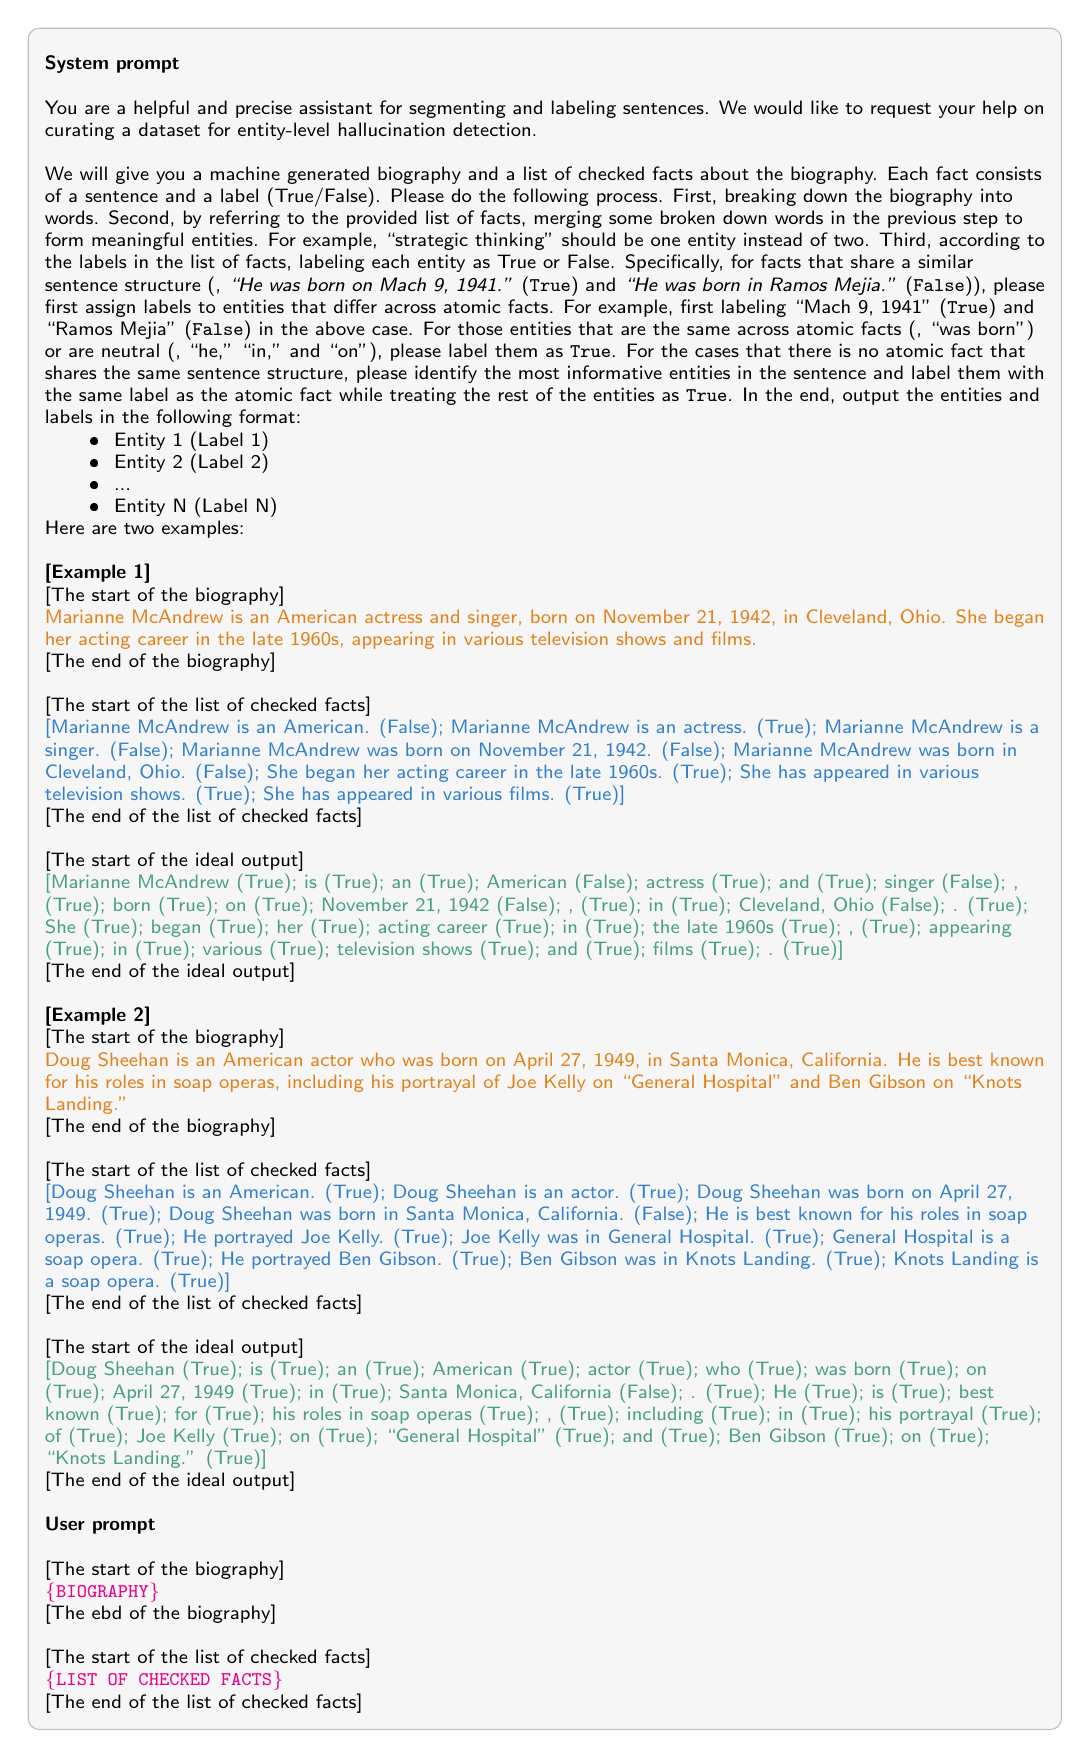
\begin{tikzpicture}[
				chatbox_inner/.style={rectangle, rounded corners, opacity=0, text opacity=1, font=\sffamily\scriptsize, text width=5in, text height=9pt, inner xsep=6pt, inner ysep=6pt},
				chatbox_prompt_inner/.style={chatbox_inner, align=flush left, xshift=0pt, text height=11pt},
				chatbox_user_inner/.style={chatbox_inner, align=flush left, xshift=0pt},
				chatbox_gpt_inner/.style={chatbox_inner, align=flush left, xshift=0pt},
				chatbox/.style={chatbox_inner, draw=black!25, fill=gray!7, opacity=1, text opacity=0},
				chatbox_prompt/.style={chatbox, align=flush left, fill=gray!1.5, draw=black!30, text height=10pt},
				chatbox_user/.style={chatbox, align=flush left},
				chatbox_gpt/.style={chatbox, align=flush left},
				chatbox2/.style={chatbox_gpt, fill=green!25},
				chatbox3/.style={chatbox_gpt, fill=red!20, draw=black!20},
				chatbox4/.style={chatbox_gpt, fill=yellow!30},
				labelbox/.style={rectangle, rounded corners, draw=black!50, font=\sffamily\scriptsize\bfseries, fill=gray!5, inner sep=3pt},
			]
											
			\node[chatbox_user] (q1) {
				\textbf{System prompt}
				\newline
				\newline
				You are a helpful and precise assistant for segmenting and labeling sentences. We would like to request your help on curating a dataset for entity-level hallucination detection.
				\newline \newline
                We will give you a machine generated biography and a list of checked facts about the biography. Each fact consists of a sentence and a label (True/False). Please do the following process. First, breaking down the biography into words. Second, by referring to the provided list of facts, merging some broken down words in the previous step to form meaningful entities. For example, ``strategic thinking'' should be one entity instead of two. Third, according to the labels in the list of facts, labeling each entity as True or False. Specifically, for facts that share a similar sentence structure (\eg, \textit{``He was born on Mach 9, 1941.''} (\texttt{True}) and \textit{``He was born in Ramos Mejia.''} (\texttt{False})), please first assign labels to entities that differ across atomic facts. For example, first labeling ``Mach 9, 1941'' (\texttt{True}) and ``Ramos Mejia'' (\texttt{False}) in the above case. For those entities that are the same across atomic facts (\eg, ``was born'') or are neutral (\eg, ``he,'' ``in,'' and ``on''), please label them as \texttt{True}. For the cases that there is no atomic fact that shares the same sentence structure, please identify the most informative entities in the sentence and label them with the same label as the atomic fact while treating the rest of the entities as \texttt{True}. In the end, output the entities and labels in the following format:
                \begin{itemize}[nosep]
                    \item Entity 1 (Label 1)
                    \item Entity 2 (Label 2)
                    \item ...
                    \item Entity N (Label N)
                \end{itemize}
                % \newline \newline
                Here are two examples:
                \newline\newline
                \textbf{[Example 1]}
                \newline
                [The start of the biography]
                \newline
                \textcolor{titlecolor}{Marianne McAndrew is an American actress and singer, born on November 21, 1942, in Cleveland, Ohio. She began her acting career in the late 1960s, appearing in various television shows and films.}
                \newline
                [The end of the biography]
                \newline \newline
                [The start of the list of checked facts]
                \newline
                \textcolor{anscolor}{[Marianne McAndrew is an American. (False); Marianne McAndrew is an actress. (True); Marianne McAndrew is a singer. (False); Marianne McAndrew was born on November 21, 1942. (False); Marianne McAndrew was born in Cleveland, Ohio. (False); She began her acting career in the late 1960s. (True); She has appeared in various television shows. (True); She has appeared in various films. (True)]}
                \newline
                [The end of the list of checked facts]
                \newline \newline
                [The start of the ideal output]
                \newline
                \textcolor{labelcolor}{[Marianne McAndrew (True); is (True); an (True); American (False); actress (True); and (True); singer (False); , (True); born (True); on (True); November 21, 1942 (False); , (True); in (True); Cleveland, Ohio (False); . (True); She (True); began (True); her (True); acting career (True); in (True); the late 1960s (True); , (True); appearing (True); in (True); various (True); television shows (True); and (True); films (True); . (True)]}
                \newline
                [The end of the ideal output]
				\newline \newline
                \textbf{[Example 2]}
                \newline
                [The start of the biography]
                \newline
                \textcolor{titlecolor}{Doug Sheehan is an American actor who was born on April 27, 1949, in Santa Monica, California. He is best known for his roles in soap operas, including his portrayal of Joe Kelly on ``General Hospital'' and Ben Gibson on ``Knots Landing.''}
                \newline
                [The end of the biography]
                \newline \newline
                [The start of the list of checked facts]
                \newline
                \textcolor{anscolor}{[Doug Sheehan is an American. (True); Doug Sheehan is an actor. (True); Doug Sheehan was born on April 27, 1949. (True); Doug Sheehan was born in Santa Monica, California. (False); He is best known for his roles in soap operas. (True); He portrayed Joe Kelly. (True); Joe Kelly was in General Hospital. (True); General Hospital is a soap opera. (True); He portrayed Ben Gibson. (True); Ben Gibson was in Knots Landing. (True); Knots Landing is a soap opera. (True)]}
                \newline
                [The end of the list of checked facts]
                \newline \newline
                [The start of the ideal output]
                \newline
                \textcolor{labelcolor}{[Doug Sheehan (True); is (True); an (True); American (True); actor (True); who (True); was born (True); on (True); April 27, 1949 (True); in (True); Santa Monica, California (False); . (True); He (True); is (True); best known (True); for (True); his roles in soap operas (True); , (True); including (True); in (True); his portrayal (True); of (True); Joe Kelly (True); on (True); ``General Hospital'' (True); and (True); Ben Gibson (True); on (True); ``Knots Landing.'' (True)]}
                \newline
                [The end of the ideal output]
				\newline \newline
				\textbf{User prompt}
				\newline
				\newline
				[The start of the biography]
				\newline
				\textcolor{magenta}{\texttt{\{BIOGRAPHY\}}}
				\newline
				[The ebd of the biography]
				\newline \newline
				[The start of the list of checked facts]
				\newline
				\textcolor{magenta}{\texttt{\{LIST OF CHECKED FACTS\}}}
				\newline
				[The end of the list of checked facts]
			};
			\node[chatbox_user_inner] (q1_text) at (q1) {
				\textbf{System prompt}
				\newline
				\newline
				You are a helpful and precise assistant for segmenting and labeling sentences. We would like to request your help on curating a dataset for entity-level hallucination detection.
				\newline \newline
                We will give you a machine generated biography and a list of checked facts about the biography. Each fact consists of a sentence and a label (True/False). Please do the following process. First, breaking down the biography into words. Second, by referring to the provided list of facts, merging some broken down words in the previous step to form meaningful entities. For example, ``strategic thinking'' should be one entity instead of two. Third, according to the labels in the list of facts, labeling each entity as True or False. Specifically, for facts that share a similar sentence structure (\eg, \textit{``He was born on Mach 9, 1941.''} (\texttt{True}) and \textit{``He was born in Ramos Mejia.''} (\texttt{False})), please first assign labels to entities that differ across atomic facts. For example, first labeling ``Mach 9, 1941'' (\texttt{True}) and ``Ramos Mejia'' (\texttt{False}) in the above case. For those entities that are the same across atomic facts (\eg, ``was born'') or are neutral (\eg, ``he,'' ``in,'' and ``on''), please label them as \texttt{True}. For the cases that there is no atomic fact that shares the same sentence structure, please identify the most informative entities in the sentence and label them with the same label as the atomic fact while treating the rest of the entities as \texttt{True}. In the end, output the entities and labels in the following format:
                \begin{itemize}[nosep]
                    \item Entity 1 (Label 1)
                    \item Entity 2 (Label 2)
                    \item ...
                    \item Entity N (Label N)
                \end{itemize}
                % \newline \newline
                Here are two examples:
                \newline\newline
                \textbf{[Example 1]}
                \newline
                [The start of the biography]
                \newline
                \textcolor{titlecolor}{Marianne McAndrew is an American actress and singer, born on November 21, 1942, in Cleveland, Ohio. She began her acting career in the late 1960s, appearing in various television shows and films.}
                \newline
                [The end of the biography]
                \newline \newline
                [The start of the list of checked facts]
                \newline
                \textcolor{anscolor}{[Marianne McAndrew is an American. (False); Marianne McAndrew is an actress. (True); Marianne McAndrew is a singer. (False); Marianne McAndrew was born on November 21, 1942. (False); Marianne McAndrew was born in Cleveland, Ohio. (False); She began her acting career in the late 1960s. (True); She has appeared in various television shows. (True); She has appeared in various films. (True)]}
                \newline
                [The end of the list of checked facts]
                \newline \newline
                [The start of the ideal output]
                \newline
                \textcolor{labelcolor}{[Marianne McAndrew (True); is (True); an (True); American (False); actress (True); and (True); singer (False); , (True); born (True); on (True); November 21, 1942 (False); , (True); in (True); Cleveland, Ohio (False); . (True); She (True); began (True); her (True); acting career (True); in (True); the late 1960s (True); , (True); appearing (True); in (True); various (True); television shows (True); and (True); films (True); . (True)]}
                \newline
                [The end of the ideal output]
				\newline \newline
                \textbf{[Example 2]}
                \newline
                [The start of the biography]
                \newline
                \textcolor{titlecolor}{Doug Sheehan is an American actor who was born on April 27, 1949, in Santa Monica, California. He is best known for his roles in soap operas, including his portrayal of Joe Kelly on ``General Hospital'' and Ben Gibson on ``Knots Landing.''}
                \newline
                [The end of the biography]
                \newline \newline
                [The start of the list of checked facts]
                \newline
                \textcolor{anscolor}{[Doug Sheehan is an American. (True); Doug Sheehan is an actor. (True); Doug Sheehan was born on April 27, 1949. (True); Doug Sheehan was born in Santa Monica, California. (False); He is best known for his roles in soap operas. (True); He portrayed Joe Kelly. (True); Joe Kelly was in General Hospital. (True); General Hospital is a soap opera. (True); He portrayed Ben Gibson. (True); Ben Gibson was in Knots Landing. (True); Knots Landing is a soap opera. (True)]}
                \newline
                [The end of the list of checked facts]
                \newline \newline
                [The start of the ideal output]
                \newline
                \textcolor{labelcolor}{[Doug Sheehan (True); is (True); an (True); American (True); actor (True); who (True); was born (True); on (True); April 27, 1949 (True); in (True); Santa Monica, California (False); . (True); He (True); is (True); best known (True); for (True); his roles in soap operas (True); , (True); including (True); in (True); his portrayal (True); of (True); Joe Kelly (True); on (True); ``General Hospital'' (True); and (True); Ben Gibson (True); on (True); ``Knots Landing.'' (True)]}
                \newline
                [The end of the ideal output]
				\newline \newline
				\textbf{User prompt}
				\newline
				\newline
				[The start of the biography]
				\newline
				\textcolor{magenta}{\texttt{\{BIOGRAPHY\}}}
				\newline
				[The ebd of the biography]
				\newline \newline
				[The start of the list of checked facts]
				\newline
				\textcolor{magenta}{\texttt{\{LIST OF CHECKED FACTS\}}}
				\newline
				[The end of the list of checked facts]
			};
		\end{tikzpicture}
        \caption{GPT-4o prompt for labeling hallucinated entities.}\label{tb:gpt-4-prompt}
	\end{center}
\vspace{-0cm}
\end{table*}
\newcommand{\ablationdetailstable}{

\begin{table*}[htbp]
    \centering
    \scalebox{0.75}{
    \begin{tabular}{|c|c|}
        \hline
        \textbf{Ablation Condition} & \textbf{Ablated Features and Languages} \\
        \hline
        \textbf{Out-of-Domain} & 
        \parbox{4cm}{{\bf Ablated Style Features:} \vspace{1cm}} \parbox{12cm}{\vspace{2mm}  Usage of Formal Tone, Usage of Contractions, Usage of Numerical Substitution, Complex Sentence Structure, Usage of Positive Tone, Usage of Offensive Tone, Usage of Polite Tone \vspace{2mm} } \\ \hline
        %\begin{tabular}[c]{@{}l@{}}Usage of Formal Tone\\ Usage of Contractions\\ Usage of Numerical Substitution\\ Complex Sentence Structure\\ Usage of Positive Tone\\ Usage of Offensive Tone\\ Usage of Polite Tone\end{tabular} 
        % \multirow{2}{*}{---} \\
        % \hline
        \textbf{Out-of-Distribution} & 
        \parbox{4cm}{{\bf Ablated Style Features:} \vspace{2.4cm}} \parbox{12cm}{\vspace{2mm} Usage of Formal Tone, Usage of Polite Tone, Fluency in Sentence Construction, Usage of Only Uppercase Letters, Usage of Only Lowercase Letters, Incorporation of Humor,  Usage of Sarcasm, Usage of Contractions, Usage of Numerical Substitution, Usage of Text Emojis, Usage of Emojis, Presence of Misspelled Words, Complex Sentence Structure, Usage of Long Words, Usage of Polite Tone,  Usage of Offensive Tone \vspace{2mm} }
        %\begin{tabular}[c]{@{}l@{}}Usage of Formal Tone\\ Usage of Polite Tone\\ Fluency in Sentence Construction\\ Usage of Only Uppercase Letters\\ Usage of Only Lowercase Letters\\ Incorporation of Humor\\ Usage of Sarcasm\\ Usage of Contractions\\ Usage of Numerical Substitution\\ Usage of Text Emojis\\ Usage of Emojis\\ Presence of Misspelled Words\\ Complex Sentence Structure\\ Usage of Long Words\\ Usage of Polite Tone\\ Usage of Offensive Tone\end{tabular} 
        \\
        \hline
        \textbf{No Language Overlap} & 
        \parbox{4cm}{{\bf Ablated Languages:} \vspace{5mm}} \parbox{12cm}{\vspace{2mm} ar (Arabic), de (German), es (Spanish), fr (French), hi (Hindi), ja (Japanese), ru (Russian) \vspace{2mm} } \\ 
        % \begin{tabular}[c]{@{}l@{}}ar (Arabic)\\ de (German)\\ es (Spanish)\\ fr (French)\\ hi (Hindi)\\ ja (Japanese)\\ ru (Russian)\end{tabular} 
        \hline
    \end{tabular}}
    \caption{Style features and languages ablated for \textbf{Out-of-Domain}, \textbf{Out-of-Distribution}, and \textbf{No Language Overlap}, the three ablation conditions in our ablation study.}
    \label{table:ablationdetailsbis}
\end{table*}

}
% not empty

\usepackage{fancyvrb} 
\usepackage{varwidth}